\chapter{Analiza wymagań}
Przed implementacją systemu należy przeprowadzić analizę problemu, określić wymagania systemu, zadecydować o narzędziach i technologiach niezbędnych w implementacji systemu.
W tym rozdziale zostanie najpierw opisany problem oraz koniecznie do zaimplementowania moduły, następnie postawione zostaną wymagania jakie system musi spełniać. Ostatnim krokiem będzie omówienie narzędzi i technologii koniecznych do implementacji systemu.
\section{Opis problemu}
\begin{par}
	Tematem pracy jest zaprojektowanie i implementacja systemu podejmującego decyzje w prostej grze platformowej czasu rzeczywistego.
	Moduł odpowiedzialny za optymalizację przejścia gry, oraz podejmowanie akcji powinien być oparty o zagadnienie algorytmów genetycznych.
	Celem samej gry jest dotarcie do zdefiniowanego wcześniej celu na dwuwymiarowej mapie. Wynik końcowy przejścia może zależeć od wielu parametrów - mapa może zawierać elementy dające punkty, jak i elementy prowadzące do natychmiastowego zakończenia gry (z wynikiem pozytywnym bądź negatywnym).
	Efektem pracy powinien być system pozwalający na rozwiązanie tego typu problemu bazujący na algorytmie genetycznym.
	\newline
	Ogólne wymogi dotyczące systemu:
	\begin{itemize}
		\item
			System powinien składać się z bazowego silnika gry, wzorowanego na rozwiązaniach w klasycznych grach platformowych. Ma to być jednocześnie warstwa prezentacyjna algorytmu.
			System nie powinien sztywno zakładać realizacji algorytmu na konkretnej grze platformowej, lecz być ogólnym systemem rozwiązującym gry platformowe czasu rzeczywistego.
		\item
			System powinien pozwalać zarówno na poruszanie się po mapie przez użytkownika jak i przejście w tryb treningu populacji, który na podstawie zadanych parametrów optymalizuje przejście po mapie algorytmem genetycznym.
		\item
			Do wyniku końcowego mogą być brane pod uwagę również inne zdarzenia takie jak ilość zebranych obiektów na planszy, czy czas przejścia gry.
			Funkcja przystosowania zależeć będzie od rożnych czynników, a ich modyfikacja powinna być łatwo dostępna.
		\item
			Projekt ma mieć charakter edukacyjno-badawczy. Przydatnymi narzędziami w systemie będzie prosty w obsłudze edytor map, panel konfiguracyjny w którym możemy edytować większość parametrów związanych z samym działaniem algorytmu oraz aktywny podgląd populacji i osobników.
	\end{itemize}
\end{par}

\begin{par}
	Sam pomysł stworzenia sztucznej inteligencji do gry platformowej w czasie rzeczywistym został już wcześniej powoływany do życia, m.in. jako projekt MarioAI. 
	W chwili obecnej funkcjonuje on jako turniej dla programistów. 
	Uczestnicy mogą implementować własne rozwiązania do gotowego silnika generującego losowe poziomy, oraz porównywać wyniki z innymi uczestnikami.
	Samo zgłoszenie składa się z implementacji własnej klasy odpowiedzialnej za podejmowanie decyzji.
	Strona domowa projektu znajduje się pod adresem www.marioai.org.
\end{par}

\section{Wykorzystane narzędzia i języki programowania}
\begin{par}
	\subsection{Język Java}
	Głównym celem do zrealizowania w pracy jest problem algorytmiczny i teoretyczny.
	Praca w mniejszym stopniu opiera się na wykorzystaniu konkretnej technologii, czy języka programowania, wobec czego zostały wykorzystane popularne narzędzia i języki programowania.
	System został napisany w języku Java oraz testowany na wirtualnej maszynie javy w wersji Java SE 7u2. Biblioteka Swing została użyta do stworzenia warstwy wizualnej programu.
	Java jest językiem programowania wysokiego poziomu zaprojektowanym i stworzonym przez Jamesa Groslinga podczas gry pracował w firmie Sun Microsystems. Pierwsza propozycja stworzenia Javy pojawiłą się w roku 1991, do głównych twórców oprócz Jamesa Groslinga zalicza się również Mike'a Sheridana oraz Patrick'a Naughtona.
	Początkowo język Java był bezpośrednio związany z firmą Sun Microsystems, która kontrolowała jego rozwój do roku 2010.
	Od tego czasu firma Sun stała się częścią korporacji Oracle, wobec czego wszelkie prawa związane z językiem Java posiada Oracle.
	Java swoją składnią przypomina język C, aczkolwiek wśród pierwowzorów wymienia się również język Smalltalk.
	Aplikacje napisane w języku Java są kompilowane do kodu bajtowego Javy (ang. java bytecode), i uruchamiane na maszynie wirtualnej, co zapewnia pewnego rodzaju bezpieczeństwo w stosunku do języka C lub C++.
	Inną dużą zaletą języka Java jest jego przenośność.
	Jedynym wymogiem uruchomienia aplikacji javowej na dowolnym systemie jest obecność wirtualnej maszyny javy (ang. JVM - Java Virtual Machine).
	Dziś większość urządzeń mobilnych posiada wirtualną maszynę javy pozwalającą na uruchamianie aplikacji napisanych w tym języku.
	::BIBLIOGRAFIA TIJ-Bruce Eckel::
	Jak pisze Bruce Eckel w swojej książce poświęconej językowi Java: ``To, co wywarło na mnie największe wrażenie, kiedy poznawałem javę, to fakt, że wśród innych celów projektantów z firmy Sun znalazła się także redukcja złożoności dla programisty. 
	To tak, jakby powiedzieć: ``Nie dbamy o nic poza zmniejszeniem czasu i trudności tworzenia porządnego kodu.''(...)''.
	Ponieważ część algorytmiczna aplikacji wymaga przeprowadzania częstych symulacji zachowania środowiska oraz przeprowadzania całego przebiegu gry, istotnym czynnikiem był czas działania krytycznych miejsc w aplikacji - głównie pętli gry, wyświetlania oraz generowania nowej populacji na podstawie poprzedniej.
	Java jako język polegający na maszynie wirtualnej posiada warstwę pośrednią która spowalnia cały proces jest wolniejsza od języka C lub C++, jednak prostota realizacji części wizualnej aplikacji oraz bardzo dobra przenośność przeważyły w wyborze języka.
	Kolejnym trafnym wyborem jeśli chodzi o język i narzędzia byłby prawdopodobnie C++ wraz z biblioteką Qt do generowania grafiki i tworzenia okienek oraz kontrolek.
	Tą samą aplikację można by zrealizować za pomocą języka Python i biblioteki PyGame/Qt do warstwy wizualizacyjnej, jednak wówczas koszt czasowy realizacji algorytmu genetycznego oraz logiki gry mógłby okazać się znacząco duży, ze względu na fakt iż Python jest językiem interpretowanym, i generalnie nie jest przeznaczony do dużych obliczeń.
	Przy konieczności realizacji prostej wersji demonstracyjnej programu opisywanego w pracy, język Python wraz z biblioteką PyGame może okazać się najszybszym do implementacji ze względu na krótki kod, dynamiczne typy zmiennych oraz bogatą kolekcję struktur takich jak listy czy mapy incydencji konieczne do realizacji algorytmu.
	Sama aplikacja korzysta z kolekcji i podstawowych struktur danych występujących w języku Java.
	\subsection{Biblioteka Swing}
	Pierwszą próbą stworzenia biblioteki graficznej javy pozwalającej na tworzenie graficznego interfejsu użytkownika była biblioteka AWT (ang. Abstract Window Toolkit).
	Fala niezadowolenia wśród programistów sprawiła iż ograniczone i mało efektowne elementy graficzne biblioteki AWT zostały zastąpione przez zbiór komponentów dziś znanych jako Swing.
	W bibliotece Swing znajdziemy większość podstawowych komponentów występujących we współczesnych systemach operacyjnych włącznie z obsługą okien, natomiast w bibliotece AWT znajdziemy obsługę zdarzeń, co w połączeniu daje nam wystarczające narzędzia do stworzenia graficznego interfejsu.
	Warto zauważyć iż Swing nie korzysta z domyślnych ustawień systemu jeśli chodzi o wygląd komponentów, dzięki czemu ten sam program wygląda identycznie na każdym systemie operacyjnym.
	Alternatywą dla biblioteki Swing może być biblioteka SWT związana z projektem Eclipse.
	W odróżnieniu do Swing, komponenty korzystają z wyglądu komponentów systemu operacyjnego.
	\subsection{Narzędzia}
	Aplikacja w całości została zrealizowana w programie Netbeans 6.9.1 wspierającym testowanie, kompilację budowanie aplikacji napisanych w języku Java.
	Innym popularnym narzędziem może być Eclipse, jednak lepsze narzędzia testujące (ang. profiler) przeważyły o wyborze pierwszej aplikacji.
\end{par}
\section{Wstępna analiza problemu}
\begin{par}
	\subsection{Sterowanie}
	\begin{par}
	Aby zrealizować część odpowiedzialną za sterowanie postacią, należy użyć klasy pośredniej pomiędzy warstwą logiki silnika gry, a warstwą komunikacji z graczem.
	Przy takim rozwiązaniu sygnały z klawiatury bądź innych urządzeń peryferyjnych są przekazywane do warstwy pośredniczącej.
	Dzięki takiemu wyjściu możemy łatwo zmienić źródło sygnałów trafiających do postaci z bezpośrednich wciśnięć klawiszy na akcje przechowywane w chromosomie.
	Warstwa pośrednia odpowiada wówczas za sterowanie postacią gracza w taki sam usystematyzowany sposób, niezależnie od źródła sygnałów. 
	Z punktu widzenia logiki gry nie ma różnicy pomiędzy sygnałami z klawiatury, a wygenerowanymi akcjami.
	\end{par}
	
	\subsection{Projekt chromosomu}
	Kolejnym ważnym elementem jest odpowiednie zaprojektowanie struktury chromosomu. 
	Dwa najbardziej trafne rozwiązania opierają się na dwóch zmiennych występujących w środowisku gry: czasie oraz pozycji gracza.
	\begin{enumerate}
	\item
	{\bf Czas który upłynął od rozpoczęcia danej instancji przejścia. }
	\begin{par}

		To rozwiązanie zakłada podejmowanie akcji w grze w zależności od czasu który upłynął od jej rozpoczęcia.
		Warto zauważyć iż nie jesteśmy ograniczeni położeniem postaci na planszy, dzięki czemu możliwe są takie operacje jak brak akcji, czy powrót do początku planszy jeśli to korzystne.
		Istotną wadą tego rozwiązania byłaby duża podatność algorytmu na zapętlanie się, lub wykonywanie dużej ilości mało przydatnych ruchów. 
		Można łatwo zauważyć że przy równym prawdopodobieństwie ruchu w lewo i prawo, postać tylko nieznacznie będzie oddalać się punktu startowego. 
		Prostym rozwiązaniem tego problemu jest przyporządkowanie pewnego prawdopodobieństwa każdej akcji, dzięki czemu możemy założyć że preferowanym kierunkiem jest np. ruch postaci w prawo, nie tracąc możliwości minimalnego ruchu w lewo jeśli to korzystne.
		Pewnym utrudnieniem może być krzyżowanie tego typu chromosomów. Ponieważ akcje postaci w większości przypadków mają sens w kontekście jej aktualnego położenia, o tyle klasyczne krzyżowanie poprzez ''cięcia'' chromosomu na dwie części może okazać się kosztowne.
		Wybranie losowego punktu przecięcia i złączenie ze sobą dwóch chromosomów nie jest dobrym rozwiązaniem.
		Po połączeniu otrzymamy niespójny ciąg ruchów, które będą miały niewiele wspólnego z aktualną pozycją gracza na mapie, wobec czego będą nieużyteczne.
		Można temu zapobiec zapewniając łączenie się chromosomów jedynie w punktach w których postać w obu momentach znajduje się w tym samym lub zbliżonym miejscu. Wyznaczenie takich punktów może okazać się kosztowne.
		Przeszukiwanie punktów wspólnych można zrealizować w czasie $O(n*log_2n)$ najpierw sortując tablice obu osobników odpowiadające za ruch w chromosomie. 
		Tablice sortujemy względem współrzędnej X aktualnego położenia gracza dla każdej z akcji, a następnie liniowo przechodząc po obu tablicach osobników, szukając punktów wspólnych.
		Wówczas widać iż trzeba przechowywać dane na temat położenia w chromosomie, co jest nieco niespójne z ideą poruszania się względem czasu.
		Wstępny schemat takiego rozwiązania mógłby wówczas wyglądać tak jak na rysunku \ref{fig:sterowanie}.
		
		\begin{figure}[!h]
		\centering
		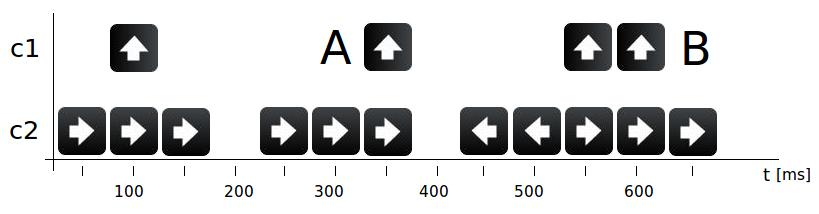
\includegraphics[width=\textwidth]{obrazki/sterowanie.jpg}
		\caption{Sterowanie względem czasu.}
		\label{fig:sterowanie}
		\end{figure}
		
		Tablice c1, c2 oznaczają odpowiednio tablicę odpowiadającą za akcje specjalne (np. skok), oraz tablicę odpowiadającą jedynie za ruch kierunkowy.

		Lepszym rozwiązaniem jest realizacja krzyżowania nie poprzez klasyczne podejście, lecz modelowane statystycznie: Potomstwo nie otrzymuje bezpośrednich fragmentów chromosomu, lecz losuje za każdym razem nowe ruchy,
		natomiast chromosomy populacji rodzicielskiej zwiększają prawdopodobieństwo wylosowania najczęściej występujących ruchów.
		Schemat takiego rozwiązania zaprezentowany jest na Rys. \ref{fig:krzyżowanie}, gdzie przedstawione zostało krzyżowanie populacji składającej się z 3 osobników (p1,p2,p3) oraz sposób liczenia nowych prawdopodobieństw w danym punkcie chromosomu.
		Do tego rozwiązania włączamy stałą decydującą o wadze jakie ma krzyżowanie: Jeśli rodzic posiada pewną akcję A w pewnym miejscu swojego chromosomu,
		wówczas potomkowi losowana jest nowa akcja, z tą różnicą iż akcja A ma teraz prawdopodobieństwo wylosowania $p_A = p_A + p_A*k$. Jeśli populacja rodzicielska składa się z $n$ rodziców,
		oraz $m$ z nich posiada w danym momencie taką samą akcję wówczas nowe prawdopodobieństwo wylosowania akcji (tylko dla tego rozpatrywanego miejsca) wynosi 
		\begin{center}
		$p_A =  p_A + {\displaystyle\sum\limits_{i=1}^m (p_A*k)} = p_A + (p_A*k)*m$.
		\end{center}
		Dzięki takiemu podejściu zachowujemy ideę krzyżowania oraz znacznie upraszczamy cały proces.
		
		\begin{figure}[!h]
		\centering
		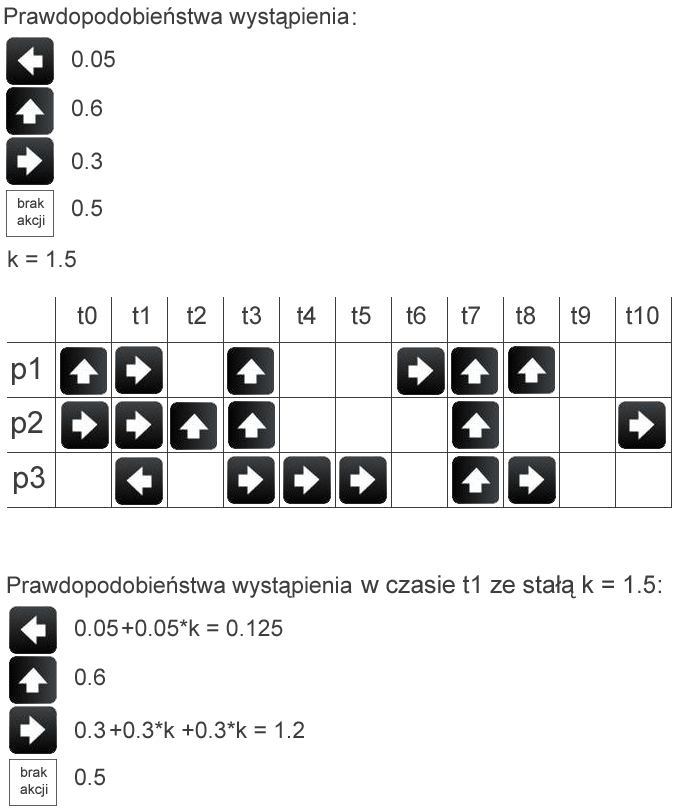
\includegraphics[width=5in]{obrazki/stat_cross.png}
		\caption{Krzyżowanie statystyczne.}
		\label{fig:krzyżowanie}
		\end{figure}

	\end{par}
	\item
	{\bf Aktualna pozycja gracza.}
	\begin{par}
		O ile poprzednie rozwiązanie dawało większą swobodę ruchu po mapie, to było jednak mało optymalne pod względem osiągania szybko dobrych wyników.
		Jeśli założymy iż akcje przechowywane w chromosomie mają być aktywowane w momencie osiągnięcia przez gracza danej pozycji na osi X mapy, wówczas uprościmy cały mechanizm krzyżowania (już nie musimy szukać punktów wspólnych, gdyż dwa dowolne indeksy w obu tablicach $i,j$ gwarantują nam takie samo położenie gracza na mapie gdy $i=j$.
		Oprócz tego przy założeniu że planszę da się rozwiązać poruszając się tylko w prawo upraszcza to większość operacji w algorytmie.
		Innym udogodnieniem będzie uproszczenie samego typu przechowywanych danych. Ponieważ rezygnujemy z postojów i ruchu w lewo, równie dobrze możemy zrezygnować z tablicy przechowującej te informacje.

		\begin{par}
		\begin{figure}[!h]
		\centering
		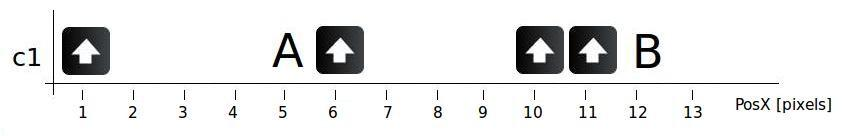
\includegraphics[width=\textwidth]{obrazki/sterowanie2.jpg}
		\caption{Sterowanie względem pozycji gracza.}
		\label{fig:sterowanie2}
		\end{figure}
		\end{par}

		To podejście posiada jednak kilka poważnych wad i wymaga pewnych ograniczających założeń.
		Plansza musi być ukierunkowana, i być rozwiązywalna przy ciągłym ruchu w określonym kierunku.
		Jest to rozwiązanie działające jedynie dla bardzo wąskiej grupy gier platformowych (np. wspomniane wcześniej Super Mario Brothers).
		Przeniesienie systemu do zastosowania w grze platformowej o nieco innym schemacie ruchu (np. rozwiązywania labiryntu) może okazać się trudne i wymagające dużych zmian w samym algorytmie.
		Jeśli chcemy tego uniknąć i traktować system bardziej ogólnie, lepiej jest skorzystać z pierwszego podejścia.
	\end{par}
	\end{enumerate}
	\FloatBarrier
\end{par}
\section{Moduł silnika i symulatora gry}

\subsection{Wymagania funkcjonalne}
	System nie wymaga różnicowania użytkowników ze względu na role. Wymagania funkcjonalne wyglądają następująco:
	\begin{itemize}
		\item {\bf Poruszanie się w środowisku gry za pomocą klawiatury.}
		\newline
		Podstawowym wymogiem systemu jest implementacja silnika prostej gry platformowej pozwalającego na poruszanie się postacią po mapie.
		Sterowanie zrealizowane powinno być intuicyjne i analogiczne do przyjętych rozwiązań w grach platformowych.
		Ponieważ oprawa graficzna nie jest priorytetem w projekcie, wystarczy prosta reprezentacja obiektów za pomocą prostokątów.
		\item {\bf Wczytanie mapy do środowiska gry.}
		\newline
		System powinien pozwalać na wczytywanie map z plików tekstowych do bieżącego środowiska symulującego przebieg gry.
		Wówczas bieżąca gra zostaje przerwana i inicjowany jest nowy przebieg gry na nowowczytanej mapie.
		\item {\bf Wczytanie nowej logiki do środowiska gry.}
		\newline
		Ponieważ system powinien być ogólnym systemem rozwiązującym gry platformowe, dostępnych powinno być kilka przykładowych gier,
		różniących się między sobą pod względem logiki. Podobnie jak w powyższym przypadku bieżąca gra powinna zostać przerwana i
		powinien zostać zainicjowany nowy przebieg gry z nową logiką.
		\item {\bf Przejście w tryb treningu populacji.}
		\newline
		Po przejściu w tryb treningu populacji użytkownikowi odbierana jest możliwość poruszania się postacią po ekranie.
		Jeśli nie istnieje jeszcze zainicjowana żadna populacja początkowa, następuje wylosowanie pierwszej populacji, po czym system rozpoczyna trening populacji w danym środowisku gry, zgodnie z danymi ustawieniami w systemie. Przechodzenie pomiędzy treningiem populacji a grą użytkownika powinno być możliwe w obie strony. 
		Wówczas jeśli użytkownik zainicjuje trening populacji, następnie przejdzie w tryb swobodnej gry, a ostatecznie znowu rozpocznie trening populacji, domyślną populacją jest ta która została zapisana podczas ostatniego treningu.
		\item {\bf Zainicjowane nowej populacji. }
		\newline
		Może okazać się koniecznie zainicjowanie nowej populacji podczas działania systemu, np. gdy populacja wpadła w stagnację.
		Inicjowanie nowej populacji podczas zmiany logiki, ustawień bądź wczytywania mapy jest realizowane automatycznie.
		\item {\bf Otworzenie okna ustawień.}
		\newline
		System ze względu na warstwę genetyczną powinien być w łatwo konfigurowalny. Po wyświetleniu okna ustawień użytkownik ma możliwość zmiany
		poszczególnych parametrów algorytmu bądź symulacji gry.
		\item {\bf Zastosowanie nowych ustawień. }
		\newline
		Ponieważ niektóre ustawienia wymagają porzucenia aktualnego wyniku populacji i rozpoczęcia symulacji od początku (np. rozmiar chromosomu).
		Użytkownik jest o tym fakcie informowany i pytany o ponownie uruchomienie algorytmu. 
		W przypadku gdy nie jest to koniecznie, algorytm nie zostaje przerwany, a użytkownik wedle woli może to uczynić własnoręcznie.
		\item {\bf Otworzenie okna populacji. }
		\newline
		Podczas działania algorytmu powinien być możliwy podgląd aktualnej populacji. Użytkownikowi widoczna jest wówczas lista osobników, oraz krótki opis każdego z nich:
		Wynik końcowy, ilość zebranych punktów, czas działania, wartość funkcji przystosowania. Dodatkowym elementem jest możliwość przerwania aktualnego przebiegu gry i uruchomienie tymczasowo nowego przebiegu dla dowolnego osobnika z listy wybranego przez użytkownika. Po zakończeniu przebiegu algorytm powraca do treningu populacji.
		\item {\bf Otworzenie okna osobnika. }
		\newline
		Bezpośrednio z okna populacji użytkownik ma możliwość podejrzenia szczegółów dotyczących osobników. Wówczas otwierane jest nowe okno zawierające wszystkie informacje na temat danego osobnika takie jak długość tablicy chromosomu bądź tekstowa reprezentacja całego chromosomu.		
		\item {\bf Przyspieszenie pracy algorytmu.}
		\newline
		Podczas treningu populacji często niepotrzebne jest użytkownikowi śledzenie ruchów algorytmu szczególnie w początkowym stadium. Aby szybciej osiągnąć wyniki działania algorytmu rozgrywka jest przyspieszana przez wstrzymanie wyświetlania grafiki na mapie. Oprócz tego opóźnienie koniecznie do osiągnięcia 60 klatek na sekundę podczas wyświetlania zostaje wyłączone - algorytm w tle przeprowadza symulacje.
	\end{itemize}
\subsection{Wymagania niefunkcjonalne}
	\begin{itemize}
	\item {\bf Prędkość działania aplikacji. }	
	\newline
	Ponieważ aplikacja wymaga przeprowadzenia wielu symulacji gry do osiągnięcia wyniku, koniecznie jest optymalne zaprojektowanie funkcji biorących udział w działaniu algorytmu genetycznego.
	\item {\bf Elastyczność. }
	\newline
	System powinien być napisany w taki sposób aby możliwe było go późniejsze rozwijanie, szczególnie jeśli chodzi o rozszerzanie systemu o nowe logiki gier.
	System musi zostać rozpatrzony jako generalny system rozwiązujący gry czasu rzeczywistego opierające się na 4 klawiszach kierunkowych i do 4 klawiszy specjalnych.
	\item {\bf Oprawa Graficzna. }
	\newline
	Oprawa graficzna samej gry nie jest istotna w systemie. Jeśli system ma być elastyczny jeśli chodzi o mechanikę gier, wprowadzenie bogatej grafiki niepotrzebne skomplikuje proces dodawania nowego typu gry do systemu. 
	Innym powodem zachowania prostej grafiki jest swoboda rozmiarów obiektów. 
	W większości gier platformowych stosowana jest grafika rastrowa która przy skalowaniu obiektów bez zachowania proporcji wygląda źle.
	Rozwiązanie tego problemu wiązałoby się z generowaniem grafiki proceduralnie bądź używaniem grafiki wektorowej, co jednak odbiega od istoty pracy.
	\end{itemize}


\subsection{Diagram przypadków użycia}
\begin{par}
	Diagram przypadków użycia został przedstawiony na Rys. \ref{fig:diagram_przypadkow}.
		\begin{figure}[!h]
		\centering
		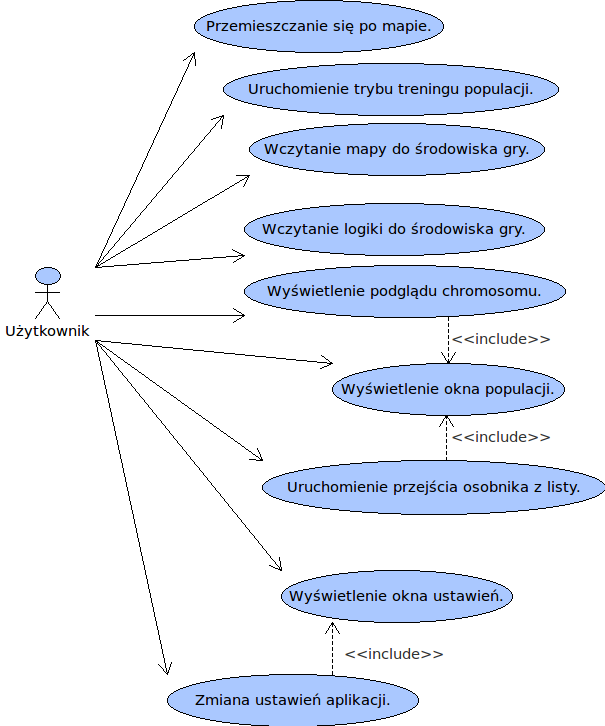
\includegraphics[width=\textwidth]{obrazki/diagram_przypadkow.png}
		\caption{Diagram przypadków użycia.}
		\label{fig:diagram_przypadkow}
		\end{figure}
		\FloatBarrier
\end{par}
\subsection{Opis tekstowy przypadków użycia}
\begin{par}
	We wszystkich przypadkach użycia aktorem jest użytkownik aplikacji.
	\begin{itemize}

	\item
	Opis przypadku użycia {\bf Przemieszczanie się po mapie }.
	\begin{enumerate}
	\item Podstawowy ciąg zdarzeń:
		\begin{enumerate}
		\item Po uruchomieniu instancji gry w głównym oknie aplikacji wyświetlona zostaje mapa wraz ze znajdującymi się na niej obiektami.
		\item Użytkownik za pomocą klawiszy na klawiaturze przesyła dane dotyczące ruchu i akcji specjalnych do środowiska gry.
		\item Postać gracza znajdująca się w grze reaguje na żądane akcje, logika gry decyduje o reakcjach obiektów w środowisku na postępy gracza.
		\item Gracz wchodzi w kolizję z jednym z obiektów kończących grę z danym wynikiem pozytywnym bądź negatywnym.
		\item Po zakończeniu gry mapa jest ponownie wczytywana i automatycznie rozpoczynana jest nowa instancja gry.
		\end{enumerate}
	\item Alternatywne ciąg zdarzeń:
		\begin{enumerate}
		\item Użytkownik w trakcie gry uruchamia tryb treningu populacji.
		\item Użytkownik w trakcie gry wczytuje nową mapę, bądź nową logikę gry, przez co gra jest przerywana i rozpoczynana od nowa.
		\end{enumerate}
	\item Zależności czasowe:
		\begin{enumerate}
		\item Częstotliwość wykonania: Samo przemieszczanie się po mapie jest akcją o charakterze ciągłym. 
		Rozpoczynanie akcji poruszania się po mapie ze stanu treningu populacji jest bliżej nieokreślone, lecz może być wykonywane średnio 1-2 razy na minutę działania aplikacji.
		\item Typowy czas realizacji: 1 minuta.
		\item Maksymalny czas realizacji: nieokreślony.
		\end{enumerate}
	\item Wartości uzyskiwane przez aktorów po zakończeniu przypadku użycia:
		\begin{enumerate}
		\item Jeśli użytkownik zakończy tryb poruszania się po mapie przez przełączenie na tryb treningu populacji, wówczas traci kontrolę nad postacią i nie ma wpływu na akcje rozgrywane w środowisku gry.
		\end{enumerate}
	\end{enumerate}
	\item
	Opis przypadku użycia {\bf Uruchomienie trybu treningu populacji. }.
	\begin{enumerate}
	\item Podstawowy ciąg zdarzeń:
		\begin{enumerate}
		\item Podczas działania aplikacji gracz uruchamia tryb treningu populacji.
		\item Jeśli jest to pierwsze uruchomienie trybu treningu wówczas nie istnieje wcześniejsza populacja, wówczas losowana jest populacja początkowa. W przeciwnym wypadku, symulacja zaczyna się od ostatniej populacji wygenerowanej przez system. 
		\item System kolejno przeprowadza wszystkie kroki algorytmu genetycznego na bieżącej populacji.
		\item Jeśli wyświetlone jest okno widoku populacji jest ono aktualizowane po każdym przebiegu gry.
		\end{enumerate}
	\item Alternatywne ciąg zdarzeń:
		\begin{enumerate}
		\item Użytkownik wybiera w oknie populacji osobnika i przeprowadza jego tymczasową symulację w środowisku, przez co trening jest chwilowo wstrzymany. Po symulacji gry danego osobnika trening jest wznawiany od ostatniego osobnika.
		\item Użytkownik wczytuje nową logikę bądź mapę, przez co aktualny przebieg gry jest przerywany. Zostaje uruchomiona nowa gra i trening populacji jest automatycznie uruchamiany od początku.
		\item Użytkownik zmienia ustawienia algorytmu genetycznego. Jeśli są to zmiany wymagające ponownego uruchomienia gry jest wyświetlony komunikat potwierdzający operację, w innym wypadku zmiany następują bez zaburzania aktualnego przebiegu treningu.
		\item Użytkownik uruchamia tryb przyspieszonego treningu, przez co wyłączona zostaje aktualizacja stanu gry w oknie aplikacji.
		\end{enumerate}
	\item Zależności czasowe:
		\begin{enumerate}
		\item Częstotliwość wykonania: Przełączanie na trening populacji może być średnio uruchamiane 1-2 razy w ciągu minuty działania aplikacji. 
		\item Typowy czas realizacji: 10 sekund - 5 minut. Samo działanie treningu populacji stanowić może około 90\% czasu działania aplikacji.
		\item Maksymalny czas realizacji: nieokreślony.
		\end{enumerate}
	\item Wartości uzyskiwane przez aktorów po zakończeniu przypadku użycia:
		\begin{enumerate}
		\item Jeśli użytkownik uruchomi tryb poruszania się po mapie wówczas przywrócone zostaje wyświetlanie stanu gry (jeśli był włączony tryb przyspieszonego treningu). Użytkownik uzyskuje kontrolę nad postacią gracza.
		\end{enumerate}
	\end{enumerate}
	
	\item
	Opis przypadku użycia {\bf Zmiana ustawień aplikacji. }.
	\begin{enumerate}
	\item Podstawowy ciąg zdarzeń:
		\begin{enumerate}
		\item Użytkownik wyświetla okno ustawień aplikacji.
		\item W polach tekstowych użytkownik dokonuje zmian na poszczególnych parametrach aplikacji
		\item Użytkownik zatwierdza zmiany przyciskiem.
		\item System sprawdza czy zmiany nie wymagają przerwania bieżącej gry i ponownego uruchomienia algorytmu.
		\begin{enumerate}
			\item Jeśli zmiany nie wymagają ponownego uruchomienia algorytmu, zmiany zostają wprowadzone bez przerywania bieżącej instancji gry.
			\item W wypadku gdy ponowne uruchomienie jest koniecznie wyświetlone zostaje okno dialogowe.
			Użytkownik jest pytanie o ponowne uruchomienie algorytmu, ma wówczas on do dyspozycji zgodę na operację, bądź cofnięcie zmian wymagających ponownego uruchomienia.
			\item Po podjęciu decyzji okno dalej pozostaje otwarte, a zgodnie z wyborem zmiany zostają dokonane bądź nie.
		\end{enumerate}
		\item Użytkownik dalej może dokonywać zmian ustawieniach aplikacji.
		\end{enumerate}
	\item Alternatywne ciąg zdarzeń:
		\begin{enumerate}
		\item Użytkownik dokonuje zmian, lecz zamiast zatwierdzić je przyciskiem - zamyka okno ustawień. Wówczas po ponownym otwarciu ładowane są aktualne ustawienia a zmiany wprowadzone przez użytkownika nie są zapamiętywane.
		\end{enumerate}
	\item Zależności czasowe:
		\begin{enumerate}
		\item Częstotliwość wykonania: 0-5 razy w ciągu działania aplikacji.
		\item Typowy czas realizacji: 1 minuta.
		\item Maksymalny czas realizacji: nieokreślony.
		\end{enumerate}
	\item Wartości uzyskiwane przez aktorów po zakończeniu przypadku użycia:
		\begin{enumerate}
		\item brak
		\end{enumerate}
	\end{enumerate}

	\item
	Opis przypadku użycia {\bf Wyświetlenie podglądu populacji. }.
	\begin{enumerate}
	\item Podstawowy ciąg zdarzeń:
		\begin{enumerate}
		\item Podczas treningu populacji użytkownik z menu w oknie głównym gry wybiera opcję ``Population''.
		\item Okno zostaje wyświetlone, i utworzony zostaje komponent JList wypełniony aktualnymi osobnikami z populacji.
		\item Jeśli dany osobnik na liście już przeprowadził symulację, widoczne są wartości punktowe zdobyte przez danego osobnika, czas przejścia oraz wynik końcowy.
		\item Podczas działania algorytmu lista jest automatycznie aktualizowana.
		\item Użytkownik zamyka okno populacji.
		\end{enumerate}
	\item Alternatywne ciąg zdarzeń:
		\begin{enumerate}
		\item Użytkownik zaznacza osobnika i wyświetla o nim szczegóły.
		\begin{enumerate}
			\item Uruchamiany jest przypadek użycia ``Wyświetlenie podglądu chromosomu''.
		\end{enumerate}
		\item Użytkownik zaznacza osobnika i uruchamia jego przejście gry.
		\begin{enumerate}
			\item Uruchamiany jest przypadek użycia ``Uruchomienie przejścia osobnika z listy.''.
		\end{enumerate}
		\end{enumerate}
	\item Zależności czasowe:
		\begin{enumerate}
		\item Częstotliwość wykonania: 0-5 razy w ciągu działania aplikacji.
		\item Typowy czas realizacji: 1 minuta.
		\item Maksymalny czas realizacji: nieokreślony.
		\end{enumerate}
	\item Wartości uzyskiwane przez aktorów po zakończeniu przypadku użycia:
		\begin{enumerate}
		\item brak
		\end{enumerate}
	\end{enumerate}
	\item
	Opis przypadku użycia {\bf Wyświetlenie podglądu chromosomu. }.
	\begin{enumerate}
	\item Podstawowy ciąg zdarzeń:
		\begin{enumerate}
		\item Użytkownik zaznacza osobnika z listy w oknie populacji.
		\item Przyciskiem "Show details" wyświetla okno szczegółów na temat danego osobnika.
		\item Dane na temat osobnika są w postaci tekstowej - użytkownik może je skopiować do schowka.
		\item Użytkownik zamyka okno szczegółów.
		\end{enumerate}
	\item Alternatywne ciąg zdarzeń:
		\begin{enumerate}
		\item Użytkownik otwiera okna szczegółów dla kilku osobników po kolei - Otwiera się kilka osobnych okien.
		\end{enumerate}
	\item Zależności czasowe:
		\begin{enumerate}
		\item Częstotliwość wykonania: 0-5 razy w ciągu działania aplikacji.
		\item Typowy czas realizacji: 20 sekund.
		\item Maksymalny czas realizacji: nieokreślony.
		\end{enumerate}
	\item Wartości uzyskiwane przez aktorów po zakończeniu przypadku użycia:
		\begin{enumerate}
		\item brak.
		\end{enumerate}
	\end{enumerate}

	\item
	Opis przypadku użycia {\bf Uruchomienie przejścia osobnika z listy. }.
	\begin{enumerate}
	\item Podstawowy ciąg zdarzeń:
		\begin{enumerate}
		\item Użytkownik zaznacza osobnika z listy w oknie populacji.
		\item Przyciskiem "Run selected" zatwierdza wybór osobnika.
		\item Jeśli jest aktualnie przeprowadzana symulacja wówczas zostaje ona przerwana i rozpoczyna się przejście gry wybranego wcześniej osobnika.
		\item Po zakończeniu przejścia system ponownie wraca do treningu populacji i zaczyna od ostatniego osobnika.
		\end{enumerate}
	\item Alternatywne ciąg zdarzeń:
		\begin{enumerate}
		\item Użytkownik uruchamia przejście osobnika w trybie przemieszczania się po mapie. Symulacja nie zostaje wówczas przeprowadzona.
		\end{enumerate}
	\item Zależności czasowe:
		\begin{enumerate}
		\item Częstotliwość wykonania: 0-10 razy w ciągu działania aplikacji.
		\item Typowy czas realizacji: zależny od długości przejścia osobnika 1 - 40 sekund.
		\item Maksymalny czas realizacji: nieokreślony.
		\end{enumerate}
	\item Wartości uzyskiwane przez aktorów po zakończeniu przypadku użycia:
		\begin{enumerate}
		\item brak.
		\end{enumerate}
	\end{enumerate}

	\end{itemize}
\end{par}

\subsection{Diagramy czynności}
\begin{par}
		Poniżej zostaną przedstawione diagramy najistotniejszych czynności w systemie.
		\begin{figure}[!h]
		\centering
		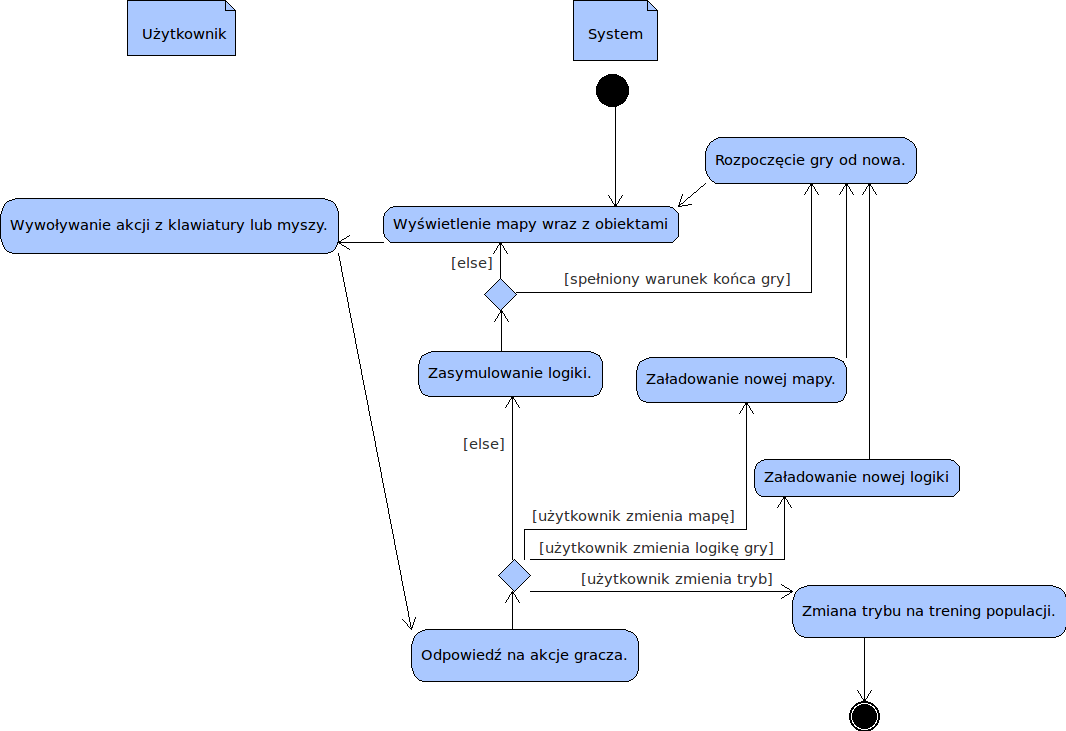
\includegraphics[width=\textwidth]{obrazki/activity_diagram.png}
		\caption{Diagram czynności ``Przemieszczanie się po mapie''.}
		\label{fig:activ1}
		\end{figure}
		\begin{figure}[!h]
		\centering
		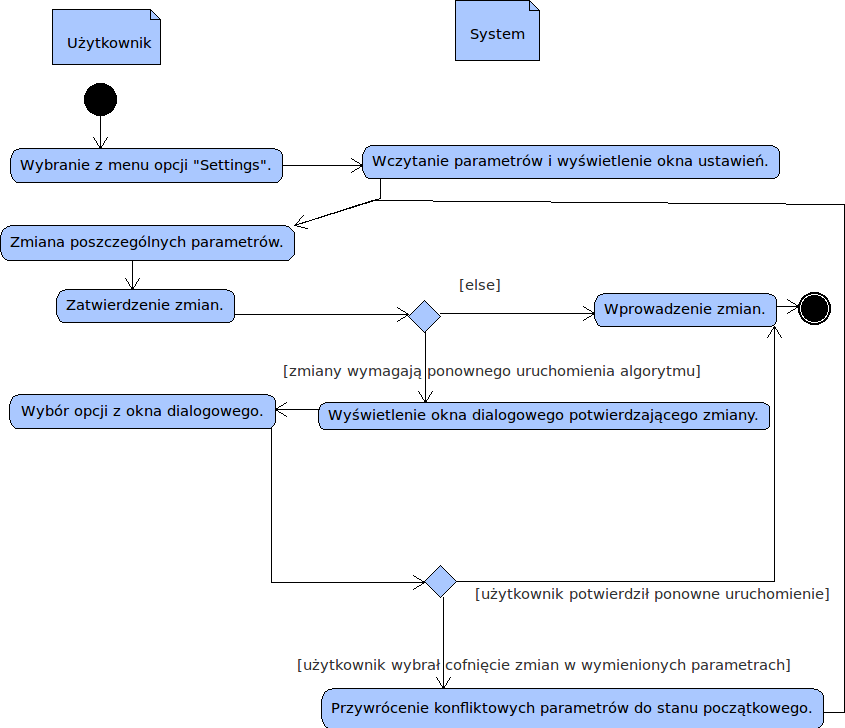
\includegraphics[width=\textwidth]{obrazki/activity_diagram_2.png}
		\caption{Diagram czynności ``Zmiana ustawień aplikacji''.}
		\label{fig:activ2}
		\end{figure}
		\FloatBarrier
\end{par}
\subsection{Diagram stanów}
\begin{par}
	System sam w sobie nie posiada wielu stanów jakie może przyjąć. Dwa główne stany to gra użytkownika w której akcje z klawiatury są interpretowane jako ruchy gracza, oraz tryb treningu populacji.
	\begin{figure}[!h]
		\centering
		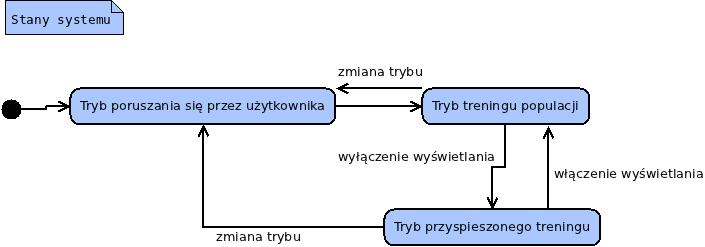
\includegraphics[width=\textwidth]{obrazki/diagram_stanow.jpg}
		\caption{Diagram czynności ``Diagram stanów systemu''.}
		\label{fig:stany}
		\end{figure}
	\FloatBarrier
	Stany dla Systemu (Rys. \ref{fig:stany}):
	Użytkownik po uruchomieniu aplikacji może poruszać się postacią po ekranie(stan ``Tryb poruszania się przez użytkownika'').
	Jeśli zmieni tryb działania systemu automatycznie przechodzi do trybu treningu (stan ``Tryb treningu populacji'').
	Będąc w stanie treningu populacji użytkownik może ponownie przejść w tym swobodnego poruszania się.
	Użytkownik może wyłączyć wyświetlanie grafiki i tym samym przyspieszyć proces treningu (stan ``Tryb przyspieszonego treningu''). 
	Ze stanu treningu przyspieszonego użytkownik może przejść do trybu poruszania się postacią po ekranie poprzez zmianę trybu, bądź do trybu treningu
	populacji poprzez włączenie wyświetlania grafiki.
\end{par}

\section{Moduł edytora map}
\subsection{Wymagania funkcjonalne}
	System nie wymaga różnicowania użytkowników ze względu na role. Wymagania funkcjonalne wyglądają następująco:
	\begin{itemize}
		
		\item {\bf Otworzenie okna edytora map. }
		\newline
		Ważnym elementem systemu jest narzędzie pozwalające tworzyć nowe mapy oraz modyfikować istniejące.
		Powinno być ono dostępne jako osobne okno edytora map.
		\item {\bf Wczytywanie mapy do edytora. }
		\newline
		Użytkownik powinien mieć możliwość edycji dowolnej wcześniej stworzonej mapy, w tym celu powinien móc z menu wybrać odpowiednią opcję pozwalającą na wczytanie pliku mapy z dysku.
		Wczytywanie może być zrealizowane analogicznie do wczytywania mapy do środowiska gry.
		\item {\bf Zapis mapy do pliku. }
		\newline
		Podobnie jak odczyt, zapis mapy powinien być dostępny dla użytkownika z menu. 
		Dzięki zapisowi mapy na dysk twardy użytkownik ma możliwość przechowywania wcześniej tworzonych map, a co ważniejsze otworzenie ich bezpośrednio w symulatorze gry.
		\item {\bf Edycja mapy za pomocą narzędzi graficznych.}
		\newline
		Edycja mapy powinna być intuicyjna i prosta nawet dla osoby nie znającej szczegółów formatu zapisu mapy. 
		Ponieważ każdy obiekt w grze posiada prostokątny obszar kolizji, edytor powinien pozwalać na łatwe tworzenie prostokątnych obiektów.
		Zrealizowane może być to przez wyznaczanie dwóch rogów prostokąta za pomocą metody ``przeciągnij i upuść''.
		Narzędzia powinny być dostępne po wybraniu odpowiedniej ikony w panelu narzędzi edytora map.
		Przydatne w edycji map mogą okazać się często używane akcje takie jak cofnięcie ostatniej zmiany, zaznaczenie elementów w edytorze i usuwanie ich, bądź czyszczenie całej mapy.
	\end{itemize}
\subsection{Wymagania niefunkcjonalne}
	\begin{itemize}
	\item {\bf Otwarty format mapy. }	
	\newline
	Istotną rzeczą może być tutaj przechowywanie mapy w pliku tekstowym. 
	O ile zapis binarny może okazać się szybszy i bardziej kompaktowy, to ważniejsze jest jednak
	umożliwienie użytkownikom edycji mapy ręcznie, bądź poprzez programy trzecie. Dzięki temu możliwe będzie generowanie np. bardzo długich losowych map.
	\end{itemize}


\subsection{Diagram przypadków użycia}
\begin{par}
	Diagram przypadków użycia został przedstawiony na Rys. \ref{fig:diagram_przypadkow_mapa}.
		\begin{figure}[!h]
		\centering
		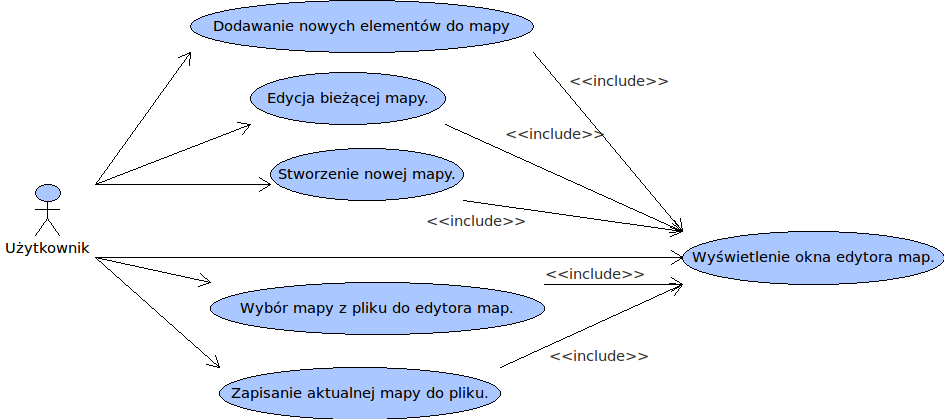
\includegraphics[width=\textwidth]{obrazki/use_case_editor.png}
		\caption{Diagram przypadków użycia modułu edytora map.}
		\label{fig:diagram_przypadkow_mapa}
		\end{figure}
		\FloatBarrier
\end{par}
\subsection{Opis tekstowy przypadków użycia}
\begin{par}
	We wszystkich przypadkach użycia aktorem jest użytkownik aplikacji.
	\begin{itemize}

	\item
	Opis przypadku użycia {\bf Edycja bieżącej mapy. }.
	\begin{enumerate}
	\item Podstawowy ciąg zdarzeń:
		\begin{enumerate}
		\item Użytkownik klika w przycisk menu dotyczący edytora map.
		\item Wyświetlone zostaje nowe okno aplikacji zawierające przyciski dotyczące edycji mapy.
		\item Do edytora map domyślnie zostaje wczytana bieżąca mapa wczytana do środowiska symulatora.
		\item Użytkownik wybiera obiekty gry użyciu przycisków znajdujących się w menu okna a następnie metodą przeciągnij-upuść rysuje prostokątne obiekty odpowiadające za obiekty w grze.
		\item Użytkownik z menu wybiera opcję zapisu mapy do pliku.
		\item Wyświetlone zostaje okno dialogowe zapisu pliku w którym użytkownik wybiera nazwę pliku.
		\item Użytkownik zamyka okno edytora map.
		\end{enumerate}
	\item Alternatywne ciąg zdarzeń:
		\begin{enumerate}
		\item Użytkownik wczytuje nowa mapę do edytora map. 
			\begin{enumerate}
			\item Wyświetlone zostaje okno dialogowe dotyczące otwarcia pliku z systemu.
			\item Wszystkie obiekty z planszy zostają usunięte, i wczytywane są nowe z wybranej wcześniej mapy.
			\end{enumerate}
		\end{enumerate}
	\item Zależności czasowe:
		\begin{enumerate}
		\item Częstotliwość wykonania: 0-5 razy w ciągu działania aplikacji.
		\item Typowy czas realizacji: 5 minut.
		\item Maksymalny czas realizacji: nieokreślony.
		\end{enumerate}
	\item Wartości uzyskiwane przez aktorów po zakończeniu przypadku użycia:
		\begin{enumerate}
		\item Użytkownik po zapisaniu stworzonej mapy do pliku ma możliwość wczytania mapy z dysku do symulatora gry i przeprowadzenia treningu populacji na nowej mapie.
		\end{enumerate}
	\end{enumerate}

	\item
	Opis przypadku użycia {\bf Stworzenie nowej mapy. }.
	\begin{enumerate}
	\item Podstawowy ciąg zdarzeń:
		\begin{enumerate}
		\item Użytkownik wybiera z menu przycisk dotyczący edytora map.
		\item Do edytora map domyślnie zostaje wczytana bieżąca mapa wczytana do środowiska symulatora.
		\item Użytkownik z panelu narzędzi edytora map wybiera usunięcie wszystkich obiektów z mapy.
		\item System usuwa obiekty z edytora map.
		\item Użytkownik za pomocą narzędzi buduje elementy nowej mapy.
		\item Użytkownik z menu wybiera opcję zapisu mapy do pliku.
		\item Wyświetlone zostaje okno dialogowe zapisu pliku w którym użytkownik wybiera nazwę pliku.
		\item Użytkownik zamyka okno edytora map.
		\end{enumerate}
	\item Zależności czasowe:
		\begin{enumerate}
		\item Częstotliwość wykonania: 0-5 razy w ciągu działania aplikacji.
		\item Typowy czas realizacji: 5 minut.
		\item Maksymalny czas realizacji: nieokreślony.
		\end{enumerate}
	\item Wartości uzyskiwane przez aktorów po zakończeniu przypadku użycia:
		\begin{enumerate}
		\item Użytkownik po utworzeniu nowej mapy ma możliwość wczytania jej w symulatorze.
		\end{enumerate}
	\end{enumerate}
	\end{itemize}
\end{par}

\subsection{Diagramy czynności}
\begin{par}
		Poniżej zostaną przedstawione diagramy najistotniejszych czynności w systemie dotyczące modułu edytora map.
		\begin{figure}[!h]
		\centering
		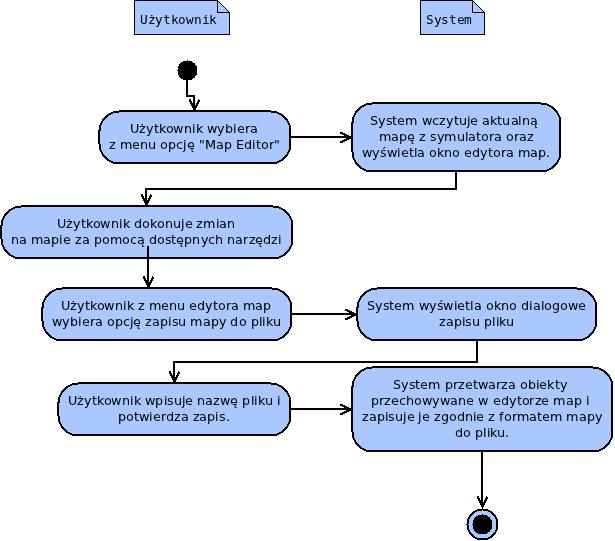
\includegraphics[width=\textwidth]{obrazki/czynnosci_edytor_map.jpeg}
		\caption{Diagram czynności ``Edycja bieżącej mapy''.}
		\label{fig:czynn_edytor_map}
		\end{figure}
		\FloatBarrier
\end{par}



\section{Diagram klas}
\begin{par}
	\begin{par}
	Diagram klas projektu przedstawiony został na rysunku \ref{fig:diagram_klas}.
	\end{par}
	\begin{figure}[!h]
	\centering
	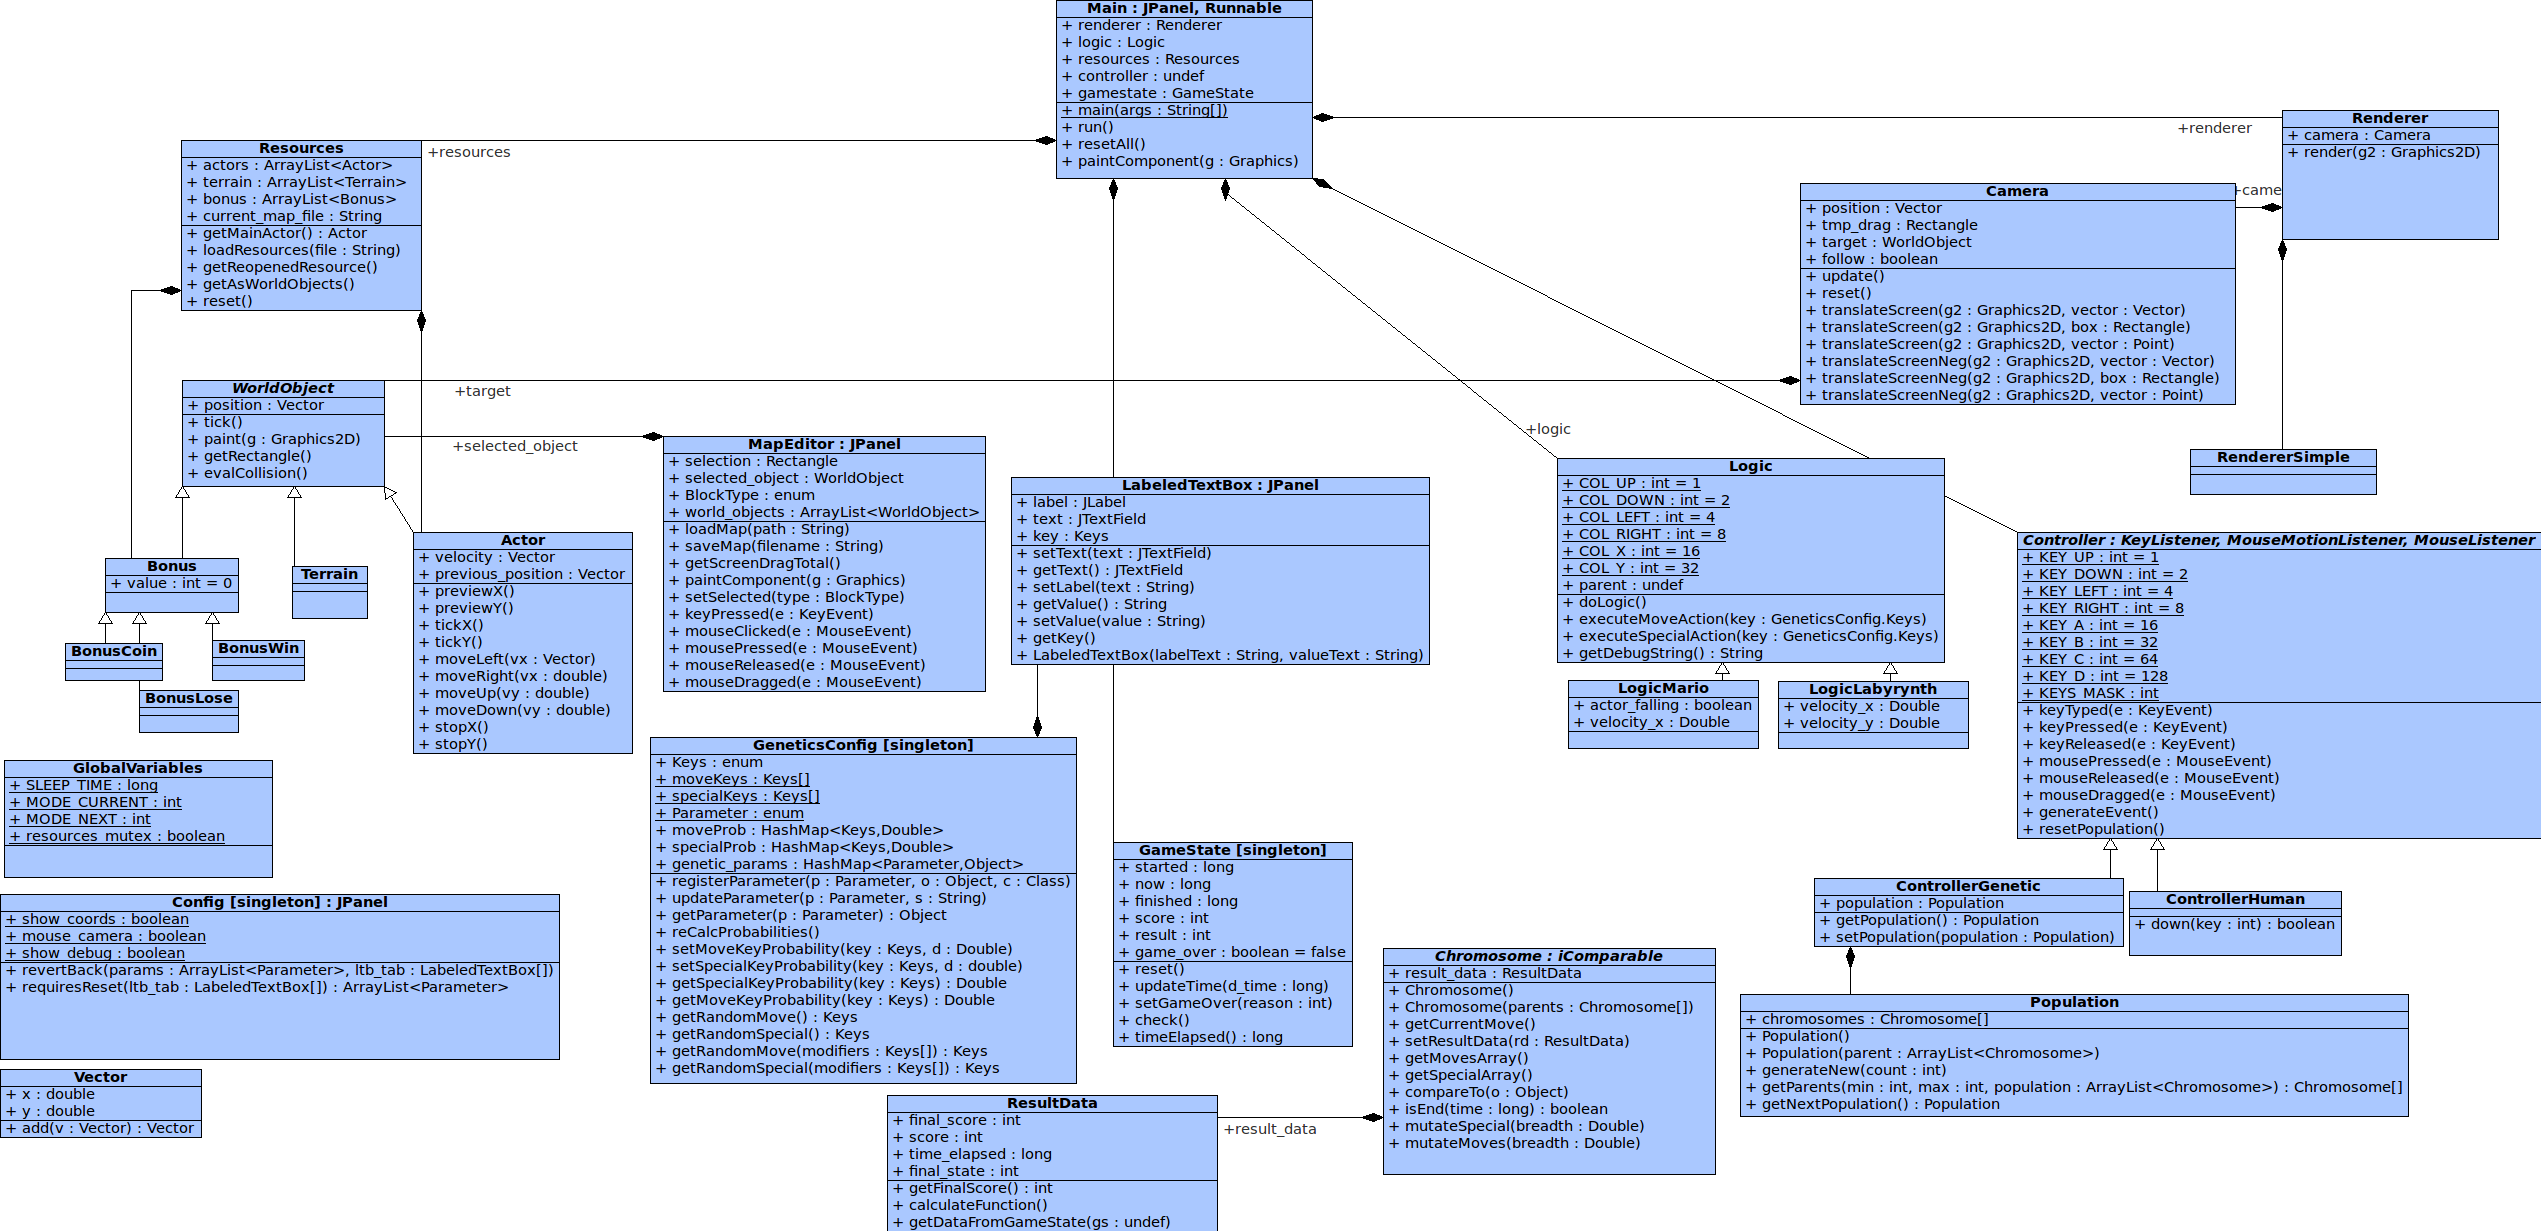
\includegraphics[height=\textheight]{obrazki/diagram_klas.png}
	\caption{Diagram Klas.}
	\label{fig:diagram_klas}
	\end{figure}
	Poniżej zostały opisane poszczególne klasy w kolejności alfabetycznej.
	\begin{enumerate}
	\item{\bf Actor }\newline
	Actor jest klasą dziedziczącą po klasie WorldObject. Reprezentuje ona obiekt postaci poruszającej się po ekranie w środowisku gry. Ponieważ instancja obiektu Actor jest przemieszczającym się obiektem niezbędne było dodanie wektora prędkości do klasy który odpowiada za zmianę pozycji w czasie. Klasa posiada metody takie jak moveLeft, moveRight, moveUp oraz moveDown pozwalające na łatwą zmianę kierunku ruchu aktora. Metody tickX, tickY aktualizują pozycje gracza. Aby wykryć kolizję możliwe jest wywołanie metody previewX (odp. previewY) która zwraca ``przyszłą'' pozycję obiektu po wykonaniu przez niego ruchu w osi X (odp. osi Y).
	\item{\bf Bonus }\newline
	Klasa Bonus jest abstrakcyjną klasą dziedziczącą po klasie WorldObject. Odpowiada ona za obiekty wpływające na przebieg gry. Kolizja aktora z obiektem powoduje wywołanie metody evalCollision, która decyduje o efekcie zdarzenia. Obiekty Bonus posiadają przypisaną wartość punktową która w zależności od typu obiektu różnie wpływa na rozgrywkę.
	\item{\bf BonusCoin }\newline
	Klasa BonusCoin reprezentuje jedynie punkty umieszczone na planszy. Kolizja z obiektem klasy BonusCoin powoduje zwiększenie licznika punków gracza bądź osobnika populacji. Poza dodaniem punktów obiekt klasy BonusCoin nie wpływa bezpośrednio na przebieg gry.
	\item{\bf BonusLose }\newline
	Obiekt klasy BonusLose reprezentuje obiekt kończący grę ze skutkiem negatywnym. Kolizja aktora z obiektem automatycznie kończy przebieg gry ze skutkiem RESULT\_LOST.
	\item{\bf BonusWin }\newline
	Obiekt klasy BonusWin stanowi cel każdej gry. Kolizja z obiektem typu BonusWin automatycznie kończy rozgrywkę ze skutkiem RESULT\_WON, co jest brane pod uwagę podczas liczenia funkcji przystosowania.
	\item{\bf Camera }\newline
	Obiekt Camera przechowuje wektor przesunięcia obrazu i jest używany do przesuwania ekranu za pomocą myszy. Jest ona wykorzystywana podczas symulacji do ``podążania'' za obiektem gracza, bądź do swobodnego przesuwania ekranu gry za pomocą myszy. Analogicznie w edytorze map użytkownik ma możliwość przesuwania ekranu za pomocą myszy, co upraszcza tworzenie dużych map. Obiekt Camera przechowuje również referencję do aktualnie śledzonego obiektu.
	Metoda update pozwala na aktualizowanie kamery wraz z przesuwaniem się postaci po ekranie.
	metody translateScreen oraz translateScreenNeg odpowiednio przesuwają ekran o żądany wektor przesunięcia.
	\item{\bf Config }\newline
	Klasa Config przechowuje zmienne dotyczące konfiguracji programu, wykorzystywane w celu wyszukiwania błędów. Przechowuje ona ustawienia wyświetlania informacji o pozycji każdego obiektu w grze, bądź dodatkowych zmiennych takich jak czas który upłynął od początku gry.
	Domyślnie informacje te nie są widoczne, lecz można je włączyć z panelu konfiguracyjnego.
	\item{\bf Controller }\newline
	Klasa Controller jest klasą pośredniczącą w wymianie informacji pomiędzy sygnałami z klawiatury, bądź akcjami zapisanymi w chromosomie, a środowiskiem gry. Odseparowuje ona obie warstwy dzięki czemu możliwe jest pisanie logiki gry, bądź reakcji na poszczególne akcje, niezależnie od źródła sygnału. Klasa Controller jest klasą abstrakcyjną i uzupełnia interfejsy takie jak KeyListener, MouseListener, MouseMotionListener (tym samym implementuje wszystkie związane z nimi metody), dzięki czemu wszelkie zdarzenia wywołane w oknie gry zostają przechwycone i odpowiednio obsłużone. Klasa Controller posiada również zmienne całkowite które są kolejnymi potęgami 2, związane jest to z optymalizacją przechwytywania ruchów z klawiatury - każde wciśnięcie klawisza ustawia odpowiedni bit.
	\item{\bf ControllerHuman }\newline
	Klasa dziedzicząca po klasie Controller, nadpisuje powyższe metody, tak aby wciśnięcia klawiszy przez gracza odpowiednio poruszały postacią w grze. Posiada ona metodę down(int) która związana jest z wyżej wymienioną optymalizacją przechwytywania ruchu. Dzięki operacjom bitowym szybko sprawdzany jest stan każdego klawisza.
	\item{\bf ControllerGenetic }\newline
	Klasa dziedzicząca po klasie Controller, odpowiada za odczytywanie wygenerowanych akcji z osobników znajdujących się w populacji i odpowiednie przekazywanie ich do środowiska gry (logiki). Instancja klasy zawiera w sobie obiekt klasy Population który przechowuje całą populację osobników.
	\item{\bf Chromosome }\newline
	Chromosome jest klasą reprezentującą obiekt osobnika. Uzupełnia ona interfejs Comparable, dzięki czemu możliwe jest wykorzystanie algorytmów sortujących ze standardowej biblioteki javy. Każdy obiekt tej klasy zawiera w sobie instancje obiektu ResultData która przechowuje dane na temat wyniku gry. Klasa posiada metody takie jak mutateSpecial i mutateMoves które odpowiednio dokonują mutacji osobnika na tablicy akcji specjalnych i tablicy ruchów. Parametr breadth decyduje o ``rozległości'' mutacji, np: wartość 0.2 spowoduje mutację losowych 20\% akcji w danej tablicy chromosomu. Oprócz standardowego konstruktora klasy jest także konstruktor przyjmujący tablicę innych chromosomów. Traktowane jest to jako tworzenie nowego Chromosomu na podstawie kilku innych, czyli opisane wcześniej krzyżowanie statystyczne z grupy rodzicielskiej z poprzedniej populacji. 
	\item{\bf GameState }\newline
	Klasa GameState przechowuje aktualny stan gry, wraz ze zmiennymi takimi jak: czasy rozpoczęcia gry, aktualny oraz zakończenia (wszystkie wartości jako czasy systemowe w milisekundach), zebrane przez postać punkty bądź wartość wyliczona z funkcji przystosowania. Funkcja updateTime(d\_time) aktualizuje czas gry na podstawie faktycznego czasu który upłynął w systemie, dzięki czemu gra z punktu widzenia logiki przebiega tak samo bez względu na wydajność komputera na którym uruchamiany jest program.
	\item{\bf GeneticsConfig }\newline
	Klasa GeneticsConfig przechowuje wszystkie informacje dotyczące parametrów algorytmu genetycznego. Wartości prawdopodobieństw wylosowania akcji specjalnych (specialProb) bądź ruchu postaci (moveProb) przechowywane są w strukturach typu HashMap dostępnych w standardowych bibliotekach javy.
	Oprócz prawdopodobieństw klasa przechowuje też parametry algorytmów genetycznych takie jak rozmiar populacji, wielkość tablicy chromosomu, stałą krzyżowania, czy rozległość mutacji poszczególnych tablic. Parametry te również przechowywane są w tablicy asocjacyjnej, dzięki czemu możliwe jest odwoływanie się do nich poprzez typ wyliczeniowy ``Parameter''.
	Oprócz samych wartości przechowywany jest też typ każdego parametru. Metody registerParameter, updateParameter oraz getParameter służą do aktualizacji bądź pobierania parametrów z tablicy. Klasa oprócz przechowywania wartości posiada metody zwracające losowy ruch. Korzysta z tego głównie klasa Chromosome przy generowaniu nowych osobników.
	\item{\bf GlobalVariables }\newline
	Klasa GlobalVariables przechowuje zmienne statyczne widoczne w całym systemie takie jak aktualny tryb pracy, zmienną SLEEP\_TIME decydującą o tempie gry oraz zmienną odpowiadającą za zablokowywanie dostępu do zasobów - program jako aplikacja okienkowa korzysta z dwóch wątków wobec czego jest to koniecznie przy współdzieleniu zasobów takich jak obiekty gry.
	\item{\bf LabeledTextBox }\newline
	Jest to klasa pomocnicza przy tworzeniu interfejsu użytkownika - dzięki niej możliwe jest automatycznie generowanie par JLabel i JTextBox widocznych w oknie ustawień aplikacji.
	\item{\bf Logic }\newline
	Klasa Logic odpowiada za symulację logiki gry - głównie dotyczy to aktora i jego reakcji na różnego rodzaju akcje, gdyż jest on jedynym ruchomym obiektem w grze. Dzięki odseparowaniu logiki gry od pozostałych warstw możliwe jest proste rozszerzanie systemu o własne reguły gry. Klasa posiada metodę doLogic która jest cyklicznie wykonywana w każdej pętli gry. Oprócz tego metody executeMoveAction oraz executeSpecialAction decydują o reakcji środowiska oraz aktora na akcje generowane przez chromosom, bądź użytkownika.
	\item{\bf LogicLabirynth }\newline
	Jest to przykładowa implementacja gry, w której postać porusza się w 4 kierunkach. Klasa została rozszerzona o wartości ruchu postaci w obu osiach.
	\item{\bf LogicMario }\newline
	Podobnie jak klasa LogicLabirynth jest to prosta implementacja gry wzorowanej na grze Super Mario Brothers. Pomocnicza zmienne actor\_falling pomaga w realizacji fizyki w grze (wpływie grawitacji na postać). Zmienna velocity\_x odpowiada za wartość prędkości postaci w poziomie.
	\item{\bf Main }\newline
	Klasa Main jest główną klasą w grze. Zawiera ona referencje do poszczególnych komponentów systemu takich jak silnik renderujący, logika gry, mapy gry, warstwy kontrolującej wykonywanie akcji oraz bieżącego stanu gry.
	Podczas uruchomienia aplikacji uruchamiana jest metoda main(String[]) która inicjuje wszystkie koniecznie komponenty i wyświetla okno aplikacji.
	Klasa uzupełnia interfejs Runnable, dzięki czemu działa jako osobny wątek. Oprocz tego klasa Main dziedziczy po klasie JPanel i nadpisuje metodę painComponent(Graphics), dzięki czemu możliwe jest stworzenie warstwy wizualizacyjnej dla środowiska gry.
	\item{\bf MapEditor }\newline
	Klasa MapEditor podobnie jak klasa Main dziedziczy po klasie JPanel. Zawiera ona listę obiektów niezależną od obiektów istniejących w symulatorze gry. Metoda loadMap pozwala na wczytanie mapy z pliku na dysku, metoda saveMap służy do zapisu aktualnie edytowanej mapy do pliku tekstowego. Klasa uzupełnia interfejsy MouseListener oraz MouseMotionListener przez co nadpisuje metody służące do obsługi zdarzeń. 
	\item{\bf Population }\newline
	Klasa Population przechowuje tablicę osobników biorących udział w treningu populacji. 
	Metoda getNextPopulation odpowiada za wygenerowanie nowej populacji na podstawie wyników poprzedniej - to w niej wykonywane są wszystkie kroki związane z algorytmem genetycznym.
	Oprócz tego klasa posiada konstruktor generujący nową Populację na podstawie populacji rodzicielskiej (wspomniane wcześniej krzyżowanie statystyczne). Metoda getParents zwraca populację rodzicielską na podstawie aktualnej populacji.
	\item{\bf Renderer }\newline
	Renderer jest klasą odpowiedzialną za wyświetlanie elementów gry w oknie. Warstwa ta została odseparowana, dzięki czemu podczas dalszej rozbudowy aplikacji łatwo można zastąpić silnik renderujący na inny, bądź wprowadzić używanie tekstur do programu.
	\item{\bf RendererSimple }\newline
	Jest to prosta implementacja silnika renderującego. Głównym założeniem jest tutaj jedynie rysowanie prostokątnych obiektów, różniących się kolorami (Każda klasa dziedzicząca po WorldObject posiada inny kolor).
	\item{\bf Resources }\newline
	Klasa Resources przechowuje wszystkie obiekty świata gry. Metoda loadResources(String) interpretuje plik tekstowy przekazany w parametrze jako ścieżka na dysku i zamienia opis tekstowy mapy na obiekty w grze. Warto zauważyć iż metoda getMainActor zwraca jeden obiekt Aktora, natomiast w zasobach gry może być ich kilku (kolekcja actors jest listą). Jest to rozwiązanie mające na celu późniejsze rozwinięcie systemu np. do obsługi gry wieloosobowej.
	\item{\bf ResultData }\newline
	ResultData jest klasą pomocniczą przechowującą dane na temat przejścia gry każdego osobnika. Przechowuje ona zmienne takie jak wynik funkcji przystosowania (zmienna final\_score), ilość zebranych punktów na mapie (score), czas przejścia (time\_elapsed) oraz stan w jakim przejście się zakończyło (final\_state przyjmujący wartości RESULT\_TIMEOUT, RESULT\_WON bądź RESULT\_LOST). Oprócz tego posiada ona metodę liczącą funkcję przystosowania na podstawie parametrów w ustawieniach algorytmu genetycznego.
	\item{\bf Terrain }\newline
	Klasa Terrain jest klasą dziedziczącą po klasie WorldObject. Odpowiada za statyczny teren. Najczęściej kolizja z nim powoduje zatrzymanie ruchu, jednak zależy to od implementacji logiki gry.
	\item{\bf Vector }\newline
	Klasa pomocnicza przechowująca współrzędne punktu (typ double).
	\item{\bf WorldObject }\newline
	Klasa abstrakcyjna po której dziedziczą wszystkie elementy gry. Podstawową jej zmienną jest położenie na mapie oraz rozmiar (odpowiednio zmienne ``position'' oraz ``size'').
	Klasa posiada metodę getRectangle zwracającą obiekt Rectangle dostępny w standardowej bibliotece, dzięki czemu realizowanie kolizji pomiędzy dwoma obiektami jest realizowanie poprzez wywołanie metody intersects(Rectangle). Każdy dziedziczący po WorldObject obiekt ma do dyspozycji metodę evalCollision która decyduje o czynnościach wykonywanych podczas kolizji dwóch obiektów. Obiekty klasy WorldObject posiadają również metodę paint(Graphics) która odpowiada za rysowanie obiektu na ekranie (obiekcie Graphics).
	\end{enumerate}

\end{par}


